\chapter{Design} \label{design:design}
This chapter provides an in-depth description of the system architecture and its individual components, based heavily on the conclusions drawn from Chapter \ref{chap:analysis} \nameref{chap:analysis}. It will cover the separation of responsibility of each component as well their interactions.

\section{Scalability Design}
This section describes the architecture proposed in order to achieve a horizontally scalable system, as well as how the proposed architecture deals with possible problematic scenarios described in Section \ref{analysis-scale} \nameref{analysis-scale}.

The proposed design of the system architecture to achieve horizontal scalability is shown below in Figure \ref{fig:scalability-architecture}. The design can be split into four main components: \textbf{Nodes, Node Coordinator, Message Queue} and \textbf{Database}, the connections between these are shown in the Figure in different colours. The responsibilities, as well as the way in which the different components are connected and communicate with each other, are described in detail in the following sections.

\begin{figure}[!ht]
	\centering
	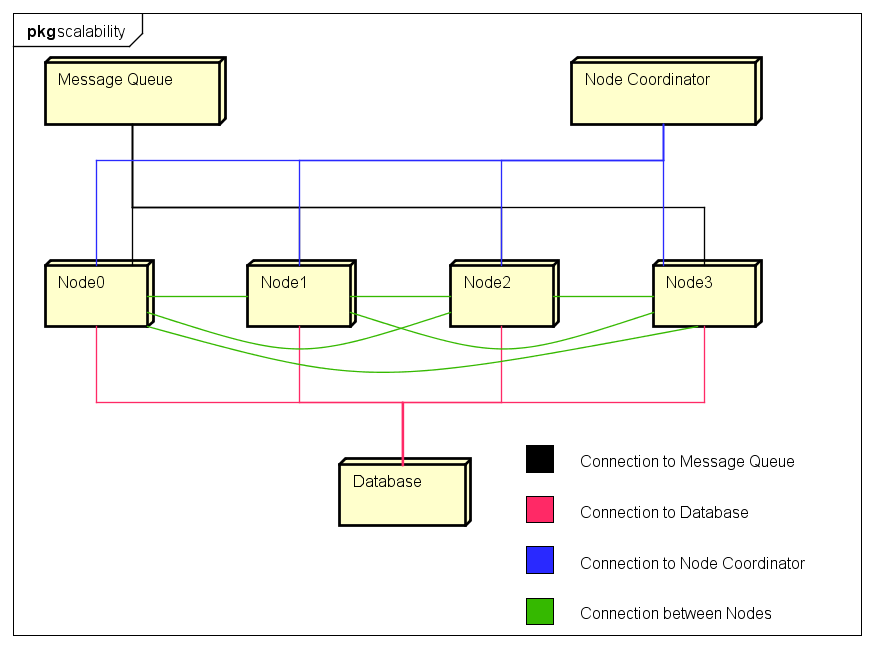
\includegraphics[width=0.7\textwidth]{figures/03_design/scalability-architecture}
    \caption{Architecture design for horizontal scalability}
    \label{fig:scalability-architecture}
\end{figure}

\subsection{Scalability Architecture Components} \label{design:scale-components}
\subsubsection{Nodes}
The Nodes form the core of the system. A node is an instance of the application containing all of the business logic. A Node's main responsibility is to dispatch messages to client devices as well as resolving groupings (such as \textit{Group} or \textit{User}, see Section \ref{design:data-layer} \nameref{design:data-layer}). The Nodes are also the system's main scalability point, as the amount of load the system can process is proportional to the number of active Nodes in the system.

Nodes are aware of each other, as they receive a list of Nodes ordered by least load from the Node Coordinator (see Section \ref{design:node-coordinator} \nameref{design:node-coordinator}).

\subsubsection{Node Coordinator} \label{design:node-coordinator}
The Node Coordinator is a simple component, whose main responsibility is to keep track of all Nodes in the system, as well as perform periodical health checks on them. Each Node should connect and announce its presence to the Node Coordinator upon start-up. The Node Coordinator also provides its connected Nodes with a list of \textit{n} least loaded Nodes.

In case of a large number of Nodes connected to the Coordinator, if Nodes requested the list of least loaded Nodes upon every request, the Coordinator could quickly become overloaded. Therefore, Nodes should cache this list for a short amount of time and update it when necessary. This is achieved by the Node only requesting a new list of least loaded Nodes after the caching time expires.

\subsubsection{Message Queue} \label{design:messagequeue}
The Message Queue component is an implementation of a message queue which is inherently scalable. For protocols that are bound to a concrete Node, for example a websocket connection, the message queue channels would correspond to individual devices connected to the Node, for example if a device with id \textit{device1} would connect to the Node, the Node would then subscribe to a channel called \textit{websocket.device1}. Any messages addressed to this device would then be pushed into this channel. This flow can be seen in Figure \ref{fig:mq-ws-device}.

\begin{figure}[!ht]
	\centering
	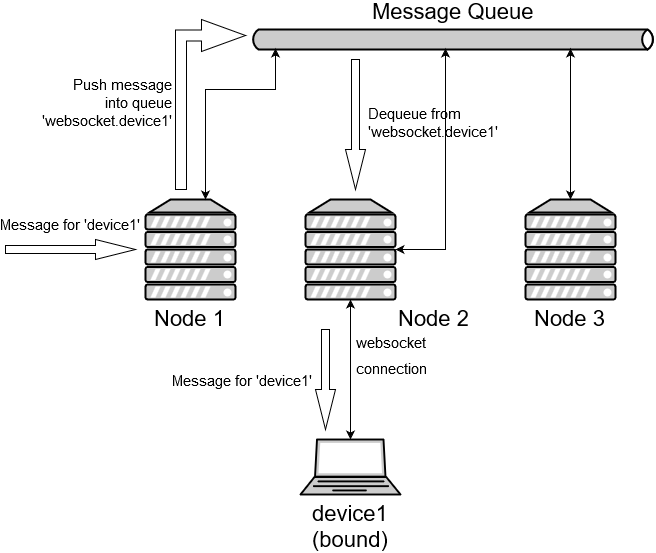
\includegraphics[width=0.7\textwidth]{figures/03_design/mq-ws-device}
    \caption{Message flow for bound device}
    \label{fig:mq-ws-device}
\end{figure}

For devices which are not bound to a concrete Node, for example mobile devices connected through FCM, the messages for the device would be pushed into the channel \textit{FCM}, from which any Node can dequeue and process it. This flow can be seen in Figure \ref{fig:mq-fcm-device}.

\begin{figure}[!ht]
	\centering
	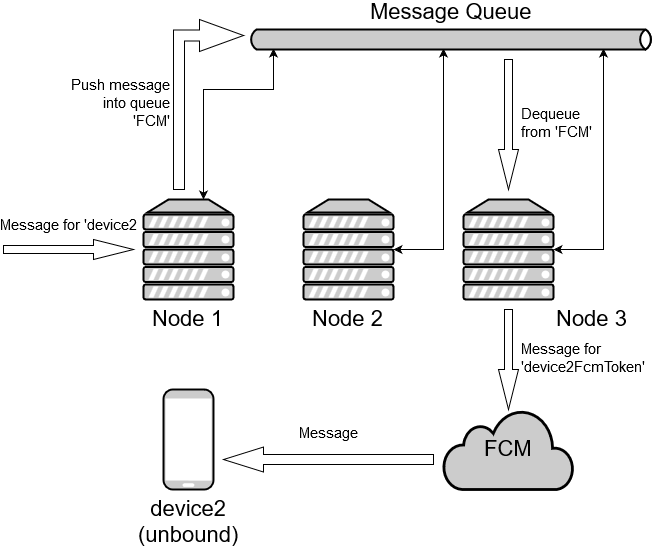
\includegraphics[width=0.7\textwidth]{figures/03_design/mq-fcm-device}
    \caption{Message flow for unbound device}
    \label{fig:mq-fcm-device}
\end{figure}

As unfolding a user into their respective devices is also an operation which does not require a specific Node to process, these are pushed to a user channel, from which the messages get distributed among all available Nodes. The equivalent can be done for groups.

\clearpage

\subsubsection{Database}
The Database component is a database layer shared between Nodes, containing all persistent data. As the database layer is fully modular, the end implementation used is up to the discretion of whoever is building the system (see Section \ref{design:database-modularity} \nameref{design:database-modularity}). However, in order to create a system that is fully scalable a scalable database solution (e.g. database cluster) is recommended.

\subsection{Problematic Scenarios and their Handling}
The system can encounter several problematic scenarios, as described in Section \ref{analysis-scale} \nameref{analysis-scale}. This section describes how the proposed architecture design handles these scenarios.

\subsubsection{Serving a large amount of clients} \label{design:serving-large-number-clients}
In this scenario, a large amount of clients is being served by the system. In order to prevent the system from becoming overwhelmed, the load must be distributed among the available Nodes in such a way that all maintain a healthy load.

The proposed architecture deals with this scenario by spreading the load using the coordination of the Nodes and the Node Coordinator. When a client tries to connect to a Node, in case the Node is above a certain load threshold, it sends the list of the least loaded Nodes to the client. The client then attempts to connect to a random Node from this list.

This resolves the issue by offloading incoming traffic onto less loaded Nodes.

\subsubsection{A large amount of clients connects at the same time}
This scenario is very similar to the one described in Section \ref{design:serving-large-number-clients} \nameref{design:serving-large-number-clients}. However, the significant difference is that in this scenario, a large number of clients are attempting to connect to the system at the same time.

The proposed architecture design deals with this scenario mostly in the same way as with the scenario \ref{design:serving-large-number-clients}. On top of that, a load balancer or DNS-level balancing should be put in place before the entry point to the system. By placing a load balancer into the system entry point or using multiple IP addresses for the DNS (Domain Name System) entry of the system, the initial connection requests can be distributed among different Nodes.

The system can handle this scenario this way also thanks to the randomization of the client connection after receiving the list of least loaded Nodes. If the clients attempted to connect to the least loaded Node, then in the case that a large number of clients connects at the same time, all would be redirected to the same Node, therefore placing it under large load. By randomly choosing between the \textit{n} least loaded Nodes, the connections are distributed among the Nodes.

\subsubsection{A large amount of messages for a single client}
This scenario describes a situation where a large number of messages are addressed to a single client.

The system handles this scenario by using a message queue which is inherently scalable. The messages for the client are expected to be sent onto different Nodes (from all the other clients), which then place them in the Message Queue. The Node to which the target client is connected to then takes these messages and passes them onto the client.

A possible bottleneck in this scenario may be the connection speed between the Node and the client, but that is unsolvable by scaling the system. However, in order to prevent the Node from getting blocked by this client and stop serving other clients connected to it, it must be able to handle each client in parallel.

\subsubsection{A node dies}
This scenario describes a situation in which a Node becomes disconnected from the system, either by crashing or connectivity issues. The system discovers that a Node has died by the Node failing a health check from the Coordinator.

The proposed design handles this situation on two levels:
\subsubsection*{Client side}
When the client loses connection to the Node it is connected to, it attempts to reconnect to it. If the reconnecting attempt also fails, it assumes the Node is no longer reachable and begins the connection process anew, connecting to a different Node.

\subsubsection*{Server side}
When a Node fails a health check, it is assumed dead and the Coordinator removes it from its connected Nodes. Any messages meant for clients connected to the now dead Node stay in the Message Queue and if the clients reconnect to a new Node within a certain message timeout period, the messages are then passed onto the clients.

\subsubsection{A message is sent to a user group with a large amount of users}
This scenario describes a situation where the system contains a group with many users. So many users in fact, that their unfolding from the group could cause an overload on the node, possibly causing it to crash.

The system handles this scenario by splitting the group into user pages of a size that can be easily handled, pushing references to these into the message queue, from where they are split across multiple nodes that process them. This flow can be seen in Figure \ref{fig:mq-group}.

\begin{figure}[!ht]
	\centering
	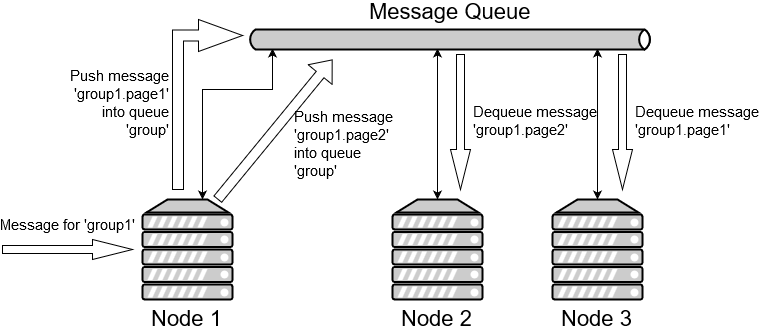
\includegraphics[width=0.9\textwidth]{figures/03_design/mq-group}
    \caption{Message flow for group unfolding (flow after user processing omitted for readability)}
    \label{fig:mq-group}
\end{figure}

\section{Architecture Design}
The system can be divided into multiple main parts\footnote{Note: These do not necessarily overlap with the modular aspects of the system.}, the highest-level of division can be into a basic four tier (or four-layered) architecture containing the following four tiers:
\begin{itemize}
\item Client Tier (Presentation Tier)
\item Collaboration Tier
\item Business Tier (Business Process Tier)
\item Data Tier
\end{itemize}

Figure ~\ref{fig:layer-arch} shows these four layers and the components belonging in each. Due to the high modularity requirements of the system, only most of the Business and part of the Collaboration Tiers belong into the core system, the Presentation and Data Tiers are to be easily interchangeable and therefore are part of the sample implementation.

A more concrete version of the tiered architecture for the full sample implementation can be seen in Figure ~\ref{fig:s-impl-arch}.

\begin{figure}[!ht]
	\centering
	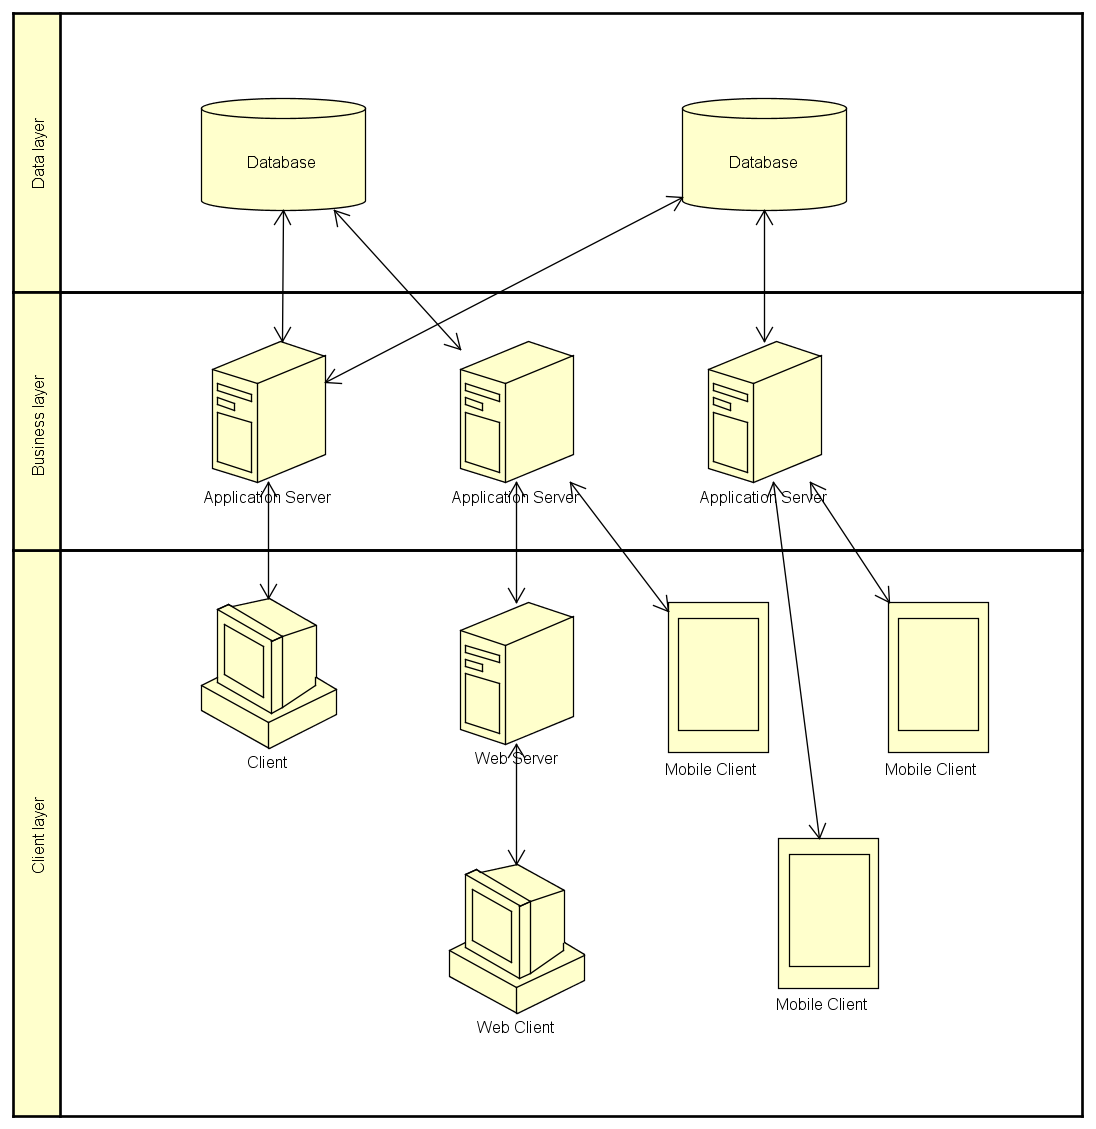
\includegraphics[width=0.8\textwidth]{figures/03_design/layer-arch}
    \caption{Four Tier basic system architecture}
    \label{fig:layer-arch}
\end{figure}

\begin{figure}[!ht]
	\centering
	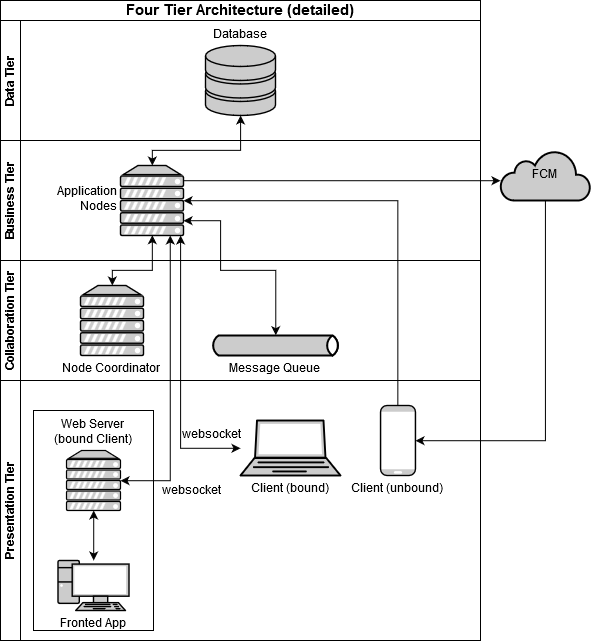
\includegraphics[width=1\textwidth]{figures/03_design/layer-arch-detail}
    \caption{Detailed Four Tier system architecture for sample implementation}
    \label{fig:s-impl-arch}
\end{figure}

\clearpage

\subsection{Data Tier} \label{design:data-layer}
The \textit{Data Tier} is used to persistently store data regarding how messages should be handled and how they are to be delivered to their intended recipient. After analysing the necessary requirements, the data to be stored has been divided into the following entities.
\begin{itemize}
\item \textbf{Group:} The Group entity represents a collection of Users, aggregated for some reason, eg. all users of an application, members of a chatroom, etc.
\item \textbf{User:} The User entity represents an end user of the application using the system. A User can belong to Groups and has Devices.
\item \textbf{Device:} The Device entity represents an end device onto which messages will be delivered. Every Device belongs to a User and is on a certain Platform.
\item \textbf{Platform:} The Platform entity represents the platform on which a Device is running and therefore determines how a message is to be delivered to that Device, eg. websocket, FCM, etc.
\end{itemize}

Due to the high modularity design required of the system, the core of the system only contains interfaces and instructions for the implementation of the data layer.

\subsubsection{Sample Implementation Data Tier}
In the sample implementation, which is part of this thesis, a relational database system will be used. The Object-Relational Mapping (ORM) implementation design of the data layer interface can be seen in Figure ~\ref{fig:orm}

\begin{figure}[H]
	\centering
	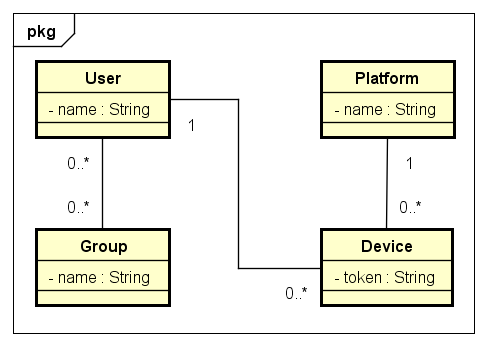
\includegraphics[width=0.6\textwidth]{figures/03_design/orm}
    \caption{Sample Implementation ORM Data Layer design}
    \label{fig:orm}
\end{figure}

\subsection{Business Tier}
The \textit{Business Tier}, also commonly known as the \textit{Business Process Tier} or \textit{Business Logic Layer}, is where all the main functions of the system are done. Here the messages are received, processed and passed along to either the message queue or the respective adapters for the target device's platform\footnote{More on adapters in Section \ref{sec:adapters}}.

Figure ~\ref{fig:msg-flow} shows a simplified representation of the flow of a message through the Business Tier. The message starts in the \textit{Client Tier}, where one of the clients sends it. After being received through the system's API it is processed and passed to the MessagingService, which communicates with the Data layer to find information on the target group, user or device and the platforms associated with them. After this, the message is passed into the message queue in the \textit{Collaboration Tier}, from which individual Nodes, subscribed to their relevant channels, receive the messages into the proper platform adapters. From here, the message is sent out to the end devices, in the \textit{Client Tier}.

\begin{figure}[H]
	\centering
	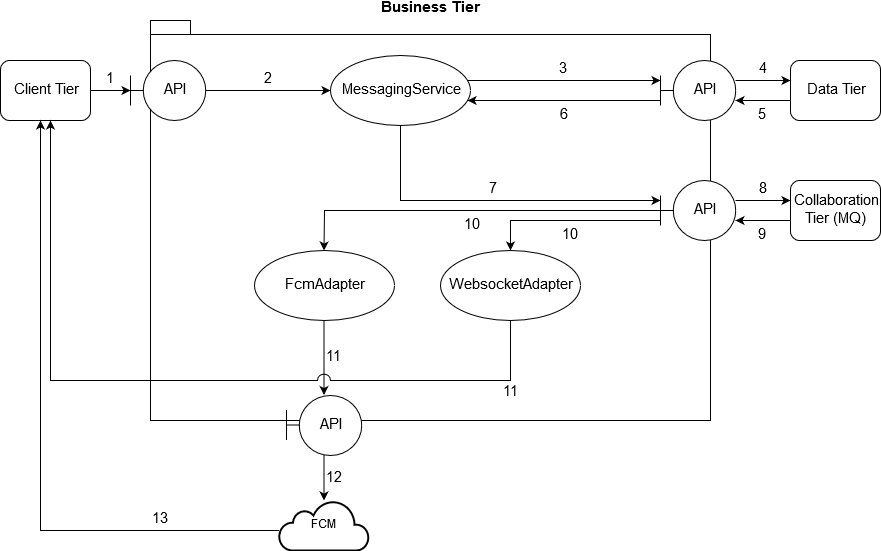
\includegraphics[width=1\textwidth]{figures/03_design/msg-flow}
    \caption{Flow of a message through the Business layer}
    \label{fig:msg-flow}
\end{figure}

\subsection{Collaboration Tier}
The \textit{Collaboration Tier} is responsible for managing information sharing among multiple instances of the \textit{Business Tier}. The \textit{Collaboration Tier} includes the Node Coordinator, which serves to keep track of active Nodes in the system, and the Message Queue, which provides a way to communicate between Nodes and distributing messages among them.

\subsection{Client Tier}
The \textit{Client Tier}, also commonly referred to as the \textit{Presentation Tier} includes all client libraries and applications that can receive and/or send messages from/to the system. Because the \textit{Client Tier} must be designed with high modularity in mind, none of it is part of the main system and the specifics of its API depend on the individual adapters\footnote{More on adapters in Section \ref{sec:adapters}} that go with it.

\subsubsection{Sample Implementation Client Tier}
The sample implementation that is part of this thesis includes an implementation of the \textit{Client Tier}, aka the client libraries, for the platforms stated in Section \ref{sec:s-impl-func-req} \nameref{sec:s-impl-func-req}.
\subsubsection*{Dektop, Server, and Mobile} \label{design:client-java}
The client library for the Desktop and Server Java platforms is a Java Archive (JAR) file, that can be included in a Java application's classpath and provides interfaces to send and receive messages to and from the system, respectively. It will be independent of any framework, such as Spring, so that it works with any Java application. Since applications for the Android mobile platform can be written in Java, the Java client library is designed in such a way that it can be used on the Android platform as well.

With real-time communication in mind, the design of the client library was made using an Event Driven architectural pattern for receiving messages through a websocket. However, keeping in mind that end applications might use a different way of consuming the messages, for example in Android's case through Firebase Cloud Messaging, connection using websockets is optional.

Figure \ref{fig:java-client-classes} shows an overview of the classes the library contains along with their external interface. For simplicity, private members of the classes have been omitted.

The most important class being \textit{MsgrClient}, which is the main point of interaction for the application using the library. It contains methods for setting up the client, sending messages, and setting up a message listener, which is an instance of the \textit{Consumer} class, from Java 8's functional API. Because in Android's ART the Groovy JSON Builder cannot be used, a \textit{Function} instance can be also set, to use custom behaviour for constructing JSON strings.

The \textit{WsSocket} class is an internal class of the library, used by the main \textit{MsgrClient} in order to process incoming and outgoing messages through a websocket connection.

Data container classes are not important to the overall architecture design, they serve simply as POJOs (Plain Old Java Objects) that envelop data, along with providing getters and setters, in order to pass the data between components in a simple, encapsulated object-oriented manner. These include classes such as \textit{DataMessageDto}, \textit{NotificationDto}, etc.

\begin{figure}[H]
	\centering
	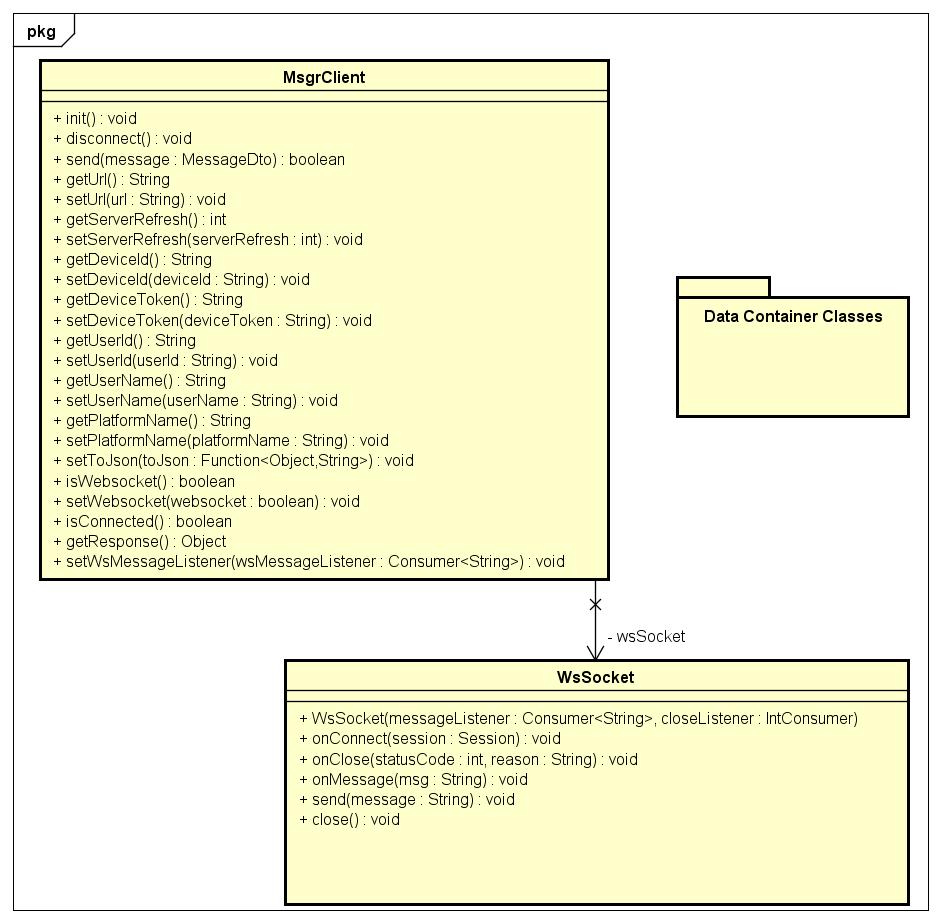
\includegraphics[width=1\textwidth]{figures/03_design/java-client-classes}
    \caption{Design of the main class components of the Java client library}
    \label{fig:java-client-classes}
\end{figure}

\subsubsection*{Web}
The Web client is a Javascript library application, its overall design very similar to the design of the Java client library described in Section \ref{design:client-java} \nameref{design:client-java} and uses websockets to communicate with the system. The Javascript library is compatible with most modern web browsers (versions: Chrome 50+, Firefox 44+, Opera Mobile 37+)\cite{fcm-web-client}.

\section{Modularity Design}

A critical part of the requirements put onto the system is its high flexibility and adaptability, based on high modularity. For this reason, the system has been designed with maximum modularity in mind. In order to achieve this, the main system is contained in a Core module, which will be the basis for any full applications with the system. Functionality and components that may be interchanged depending on the applications' needs are contained in individual modules, which can be added to the full application as further dependencies (together with the Core module). An example of an application with different modules can be seen in Figure \ref{fig:s-impl-comps}, which shows the basic module structure used in the Sample Implementation.

\begin{figure}[H]
	\centering
	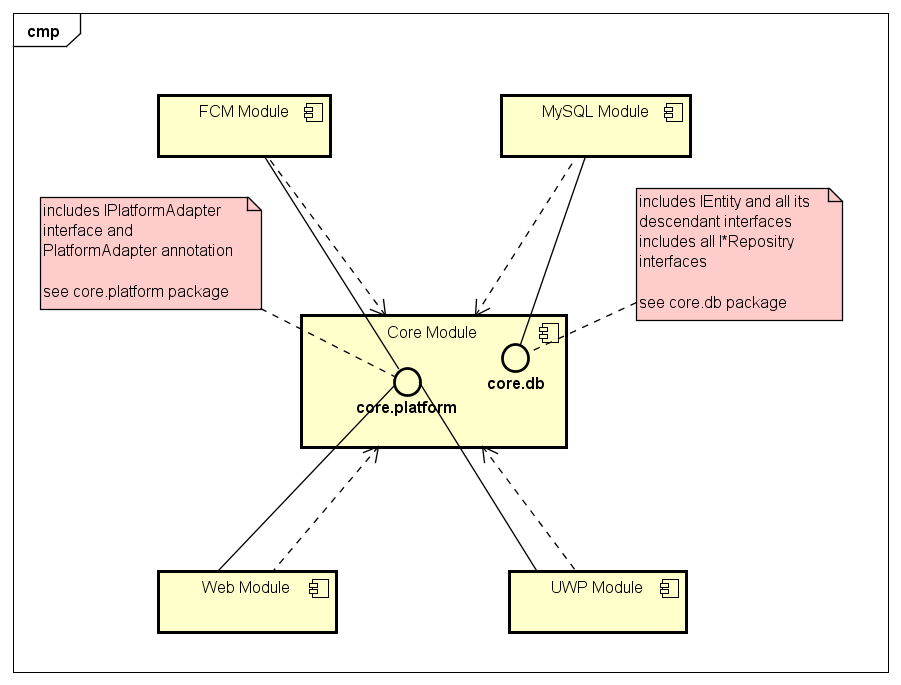
\includegraphics[width=0.9\textwidth]{figures/03_design/s-impl-comps}
    \caption{Module structure design of sample implementation}
    \label{fig:s-impl-comps}
\end{figure}

\subsection{Core Module}
The Core module, or Core library, is the heart of the entire system. The Core module provides the interfaces needed for other modules to implement the Spring Managed Beans (from now on referred to simply as Beans) that will be used across the application. 

Beans are objects whose lifecycle is managed by the Spring's IoC Container's Application Context, which means the Spring Container initializes and configures them and where needed, allows them to be injected\cite{spring-beans}. These Beans provide the main business logic of the application as well as manage the cooperation between all modules. The design of these interactions is further elaborated upon in the following sections.

The Core module also provides the business logic for basic message processing, Node health status, and core Node APIs.

\subsection{Database Modularity} \label{design:database-modularity}
The system's access to the \textit{Data Tier} has been designed in a fully modular way, so that the end deployment is not dependent on any one type or provider of database. The result of this effort for maximum freedom and interchangeability are the interfaces in the \textit{core.db} package, as seen in Figures \ref{fig:core-db-module} and \ref{fig:core-db-module-repo}.

\begin{figure}[!ht]
	\centering
	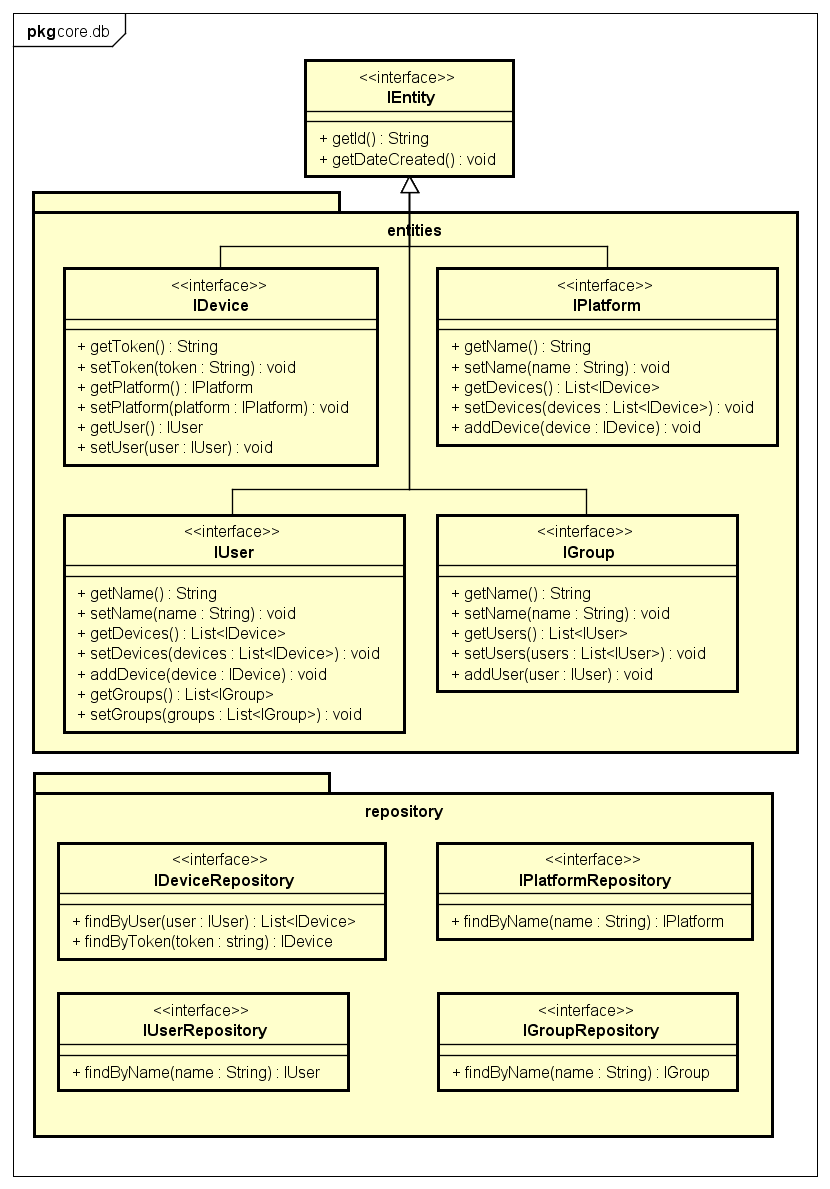
\includegraphics[width=0.95\textwidth]{figures/03_design/core-db-module}
    \caption{Interfaces for database modules in the \textit{core.db} package (Entity)}
    \label{fig:core-db-module}
\end{figure}

\begin{figure}[!ht]
	\centering
	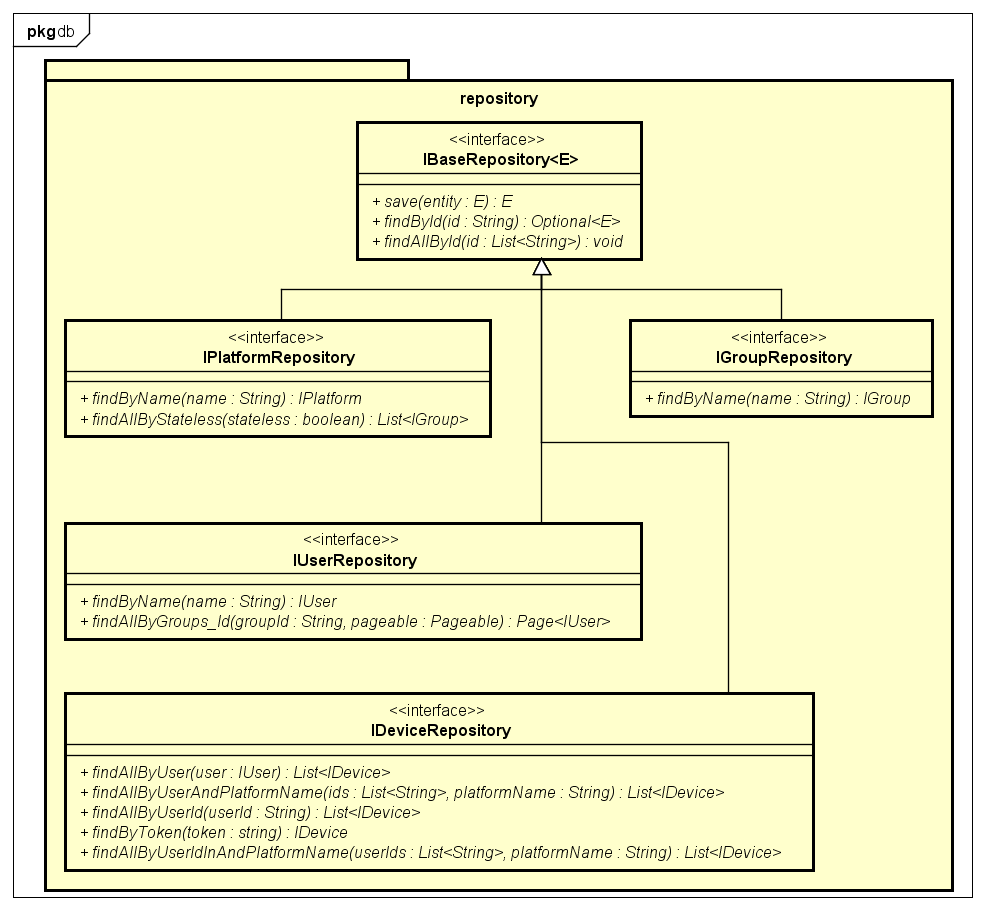
\includegraphics[width=0.95\textwidth]{figures/03_design/core-db-module-repo}
    \caption{Interfaces for database modules in the \textit{core.db} package (Repository)}
    \label{fig:core-db-module-repo}
\end{figure}

Any module that wishes to implement access to a database must create JPA Entities implementing the entity interfaces and create interfaces that extend the repository interfaces and extend Spring Data's \textit{CrudRepository} interface. This will indicate to the Spring Context to instantiate repository Beans based on these interfaces\cite{spring-repos}, which the Context will then inject into the Beans where they are used.

\subsection{Platform Modularity}
One of the key features of the system is its multi-platform support. In order to be able to support the widest possible range of platforms, the platform portion of the system had to be designed with complete modularity in mind. The results of the design choices made based on these requirements led to the creation of the \textit{IPlatformAdapter} interface and \textit{@PlatformAdapter} annotations, which can be seen in more detail in Figure \ref{fig:core-platform-module}.

\begin{figure}[!htb]
	\centering
	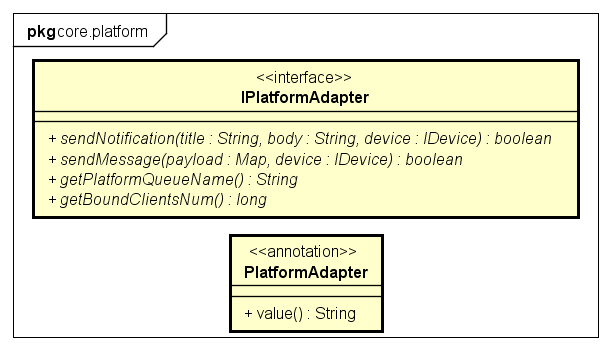
\includegraphics[width=0.95\textwidth]{figures/03_design/core-platform-module}
    \caption{Interfaces for platform modules in the \textit{core.platform} package}
    \label{fig:core-platform-module}
\end{figure}

Any module that wishes to implement support for a new platform must contain at least one Bean implementing the \textit{IPlatformAdapter} interface and annotate it with the \textit{@PlatformAdapter} annotation, which takes the platform's name as a parameter.

\subsubsection{Adapters}\label{sec:adapters}
Platform Adapters are Spring Managed Beans that implement the Core module's \textit{IPlatformAdapter} interface and are annotated with the \textit{@PlatformAdapter} annotation, which takes the platform's name as a parameter. 

Adapters are automatically found at system startup by the Core module's \textit{AdapterService} using Spring's Application Context and registered based on the platform's name, as specified in the \textit{@PlatformAdapter} annotation. The sequence of these events including an example message being sent can be seen illustrated in Figure \ref{fig:adapter-flow}

The platform adapters need to subscribe to their relevant queues/topics in the message queue, using the \textit{IReceiver} bean (see Section \ref{design:mq-modularity} \nameref{design:mq-modularity}). The timing of when to subscribe is up to the adapter, as it may differ based on the platform it is for. For example for the FCM platform, the adapter subscribes after its initialization, while the websocket adapter subscribes after a device is bound to it.

\begin{figure}[!ht]
	\centering
	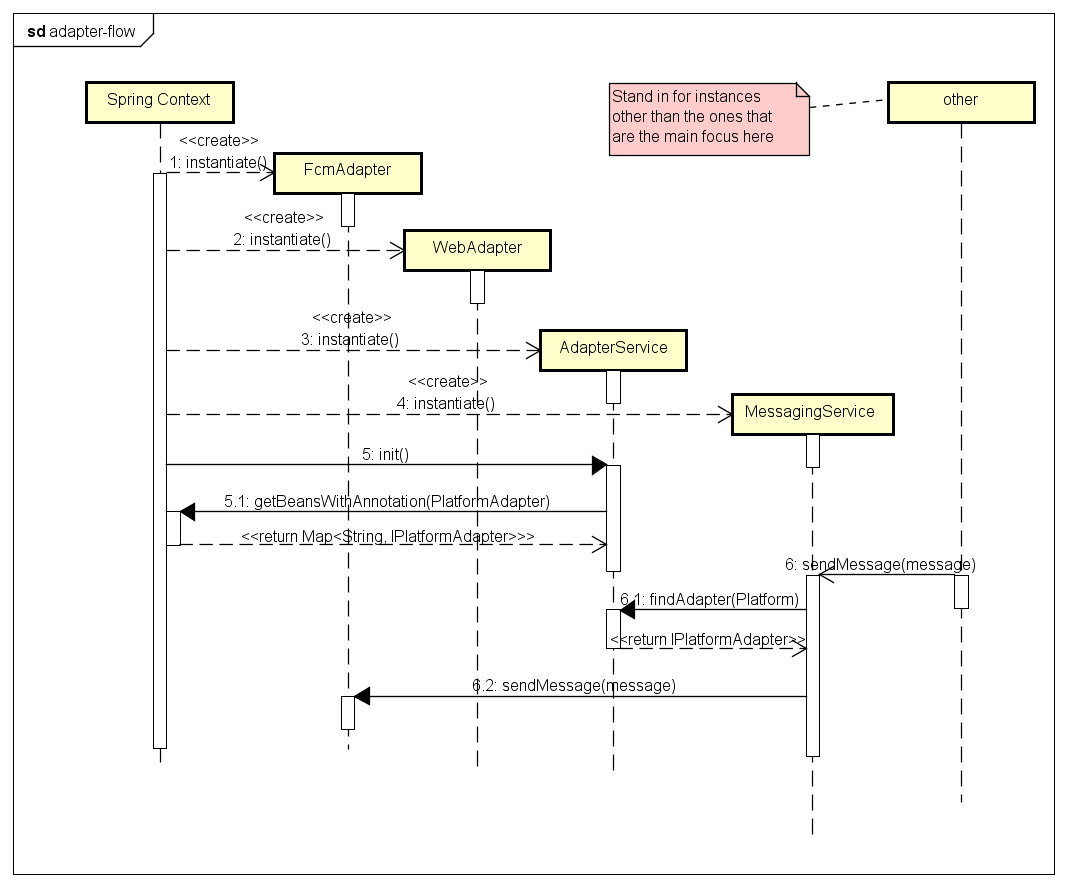
\includegraphics[width=1\textwidth]{figures/03_design/adapter-flow}
    \caption{Sequence diagram indicating the resolution process of Adapters}
    \label{fig:adapter-flow}
\end{figure}

\clearpage

\subsection{Message Queue Modularity} \label{design:mq-modularity}
The message queue portion of the application has also been designed in a modular way, so the best solution for each specific scenario can be used. Modules that would implement the message queue functionality need to implement the interfaces defined in the \textit{core.mq} package, which can be seen in Figure \ref{fig:code-mq-module}.

\begin{figure}[!ht]
	\centering
	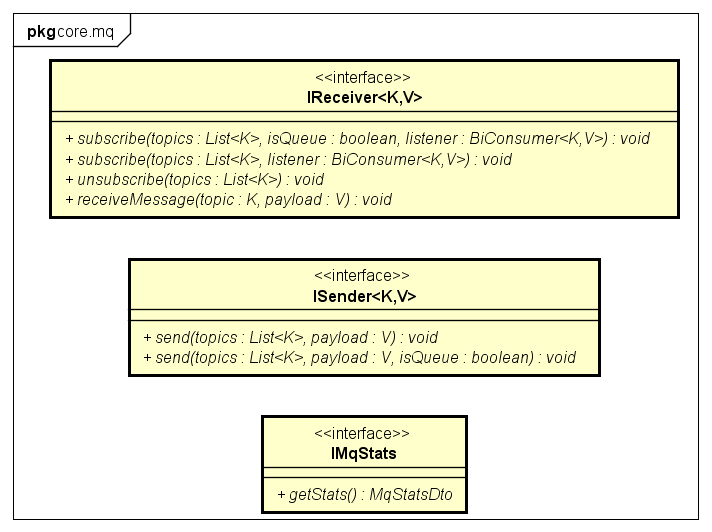
\includegraphics[width=0.9\textwidth]{figures/03_design/core-mq-module}
    \caption{Interfaces for message queue modules in the \textit{core.mq} package}
    \label{fig:code-mq-module}
\end{figure}

The message queue core package consist of three main interfaces, the \textit{ISender}, \textit{IReceiver}, and \textit{IMqStats}. The interfaces use Java generics, where \textbf{K} stands for the type of the message queue key. In most message queue implementations, this would be a String. The \textbf{V} generic stands for the type that is pushed into the message queue. While the sample implementation uses a String containing a JSON object, the use of generics in the interface allows implementations of the message queue model to use other types, for example an array of bytes as a direct serialization of Java objects.
